\documentclass[12pt,a4paper]{article}
\usepackage[latin1]{inputenc}
\usepackage{amsmath}
\usepackage{amsfonts}
\usepackage{amssymb}
\usepackage{graphicx}
\usepackage{float}
\usepackage{amsmath}
\usepackage{url}
\usepackage{hyperref}
\graphicspath{ {img/} }
\begin{document}

\title{ Open World Streaming: \linebreak
Automatic memory management in open world games without loading screens. }

\author{Alejandro Juan P�rez}

\maketitle

\newpage

\tableofcontents

\newpage

\section{Introduction}


Open world games are among the most appreciated games by players. They provide users the chance to explore a big world and they are very immersive.  Open world games grant players the freedom to take any decision and enjoy their high interaction.

As you might already know, in open world games the player usually controls an avatar over a big virtual world. So the player that controls the avatar takes its skin and, ideally, gets immersed in the virtual world.

Sure you know about some of the most famous open world games. Some of them are: \emph{Grad Theft Auto} series (by \emph{Rockstar}), \emph{The Elder Of Scrolls} series (by \emph{Bethesda}), \emph{Minecraft} (by \emph{Mojang}). These games, apart from being very famous, have all been in the top of the best-selling videogames. Let's see some examples. \emph{Minecraft} has sold 19 million copies for the PC platform and it is the most sold PC game ever. Grand Theft Auto V has sold 19 millons copies for the \emph{PS3}, making it the most sold \emph{PS3} game ever. The \emph{Eder Scrolls: Skyrim} has sold 20 millon copies for \emph{PC}, \emph{XBOX} and \emph{PS3}\cite{bestselling}.

Therefore, open world games are not only about fun, freedom and high interaction but also a promising business. And as we will see they are technologically challenging.

Despite open world games are well know, the techniques that are applied in their implementation are not. Game studios that are experienced in the implementation of open world games, like \emph{Rockstar}, keep well their secrets. The development of open world game engines requires a great investment.

The purpose of this project is to develop a game engine that will support making open world videogames. Our engine should allow the creation of games with huge worlds and avoid loading screens.

\section{Requirements}

So we are willing to make a game engine that supports the development of open world games. We are going to focus on the requirements that are more specific for open world games. And requirements that are common for most game engines will be left as secondary requirements.

\subsection{Main requirements}

We consider these requirements are the main target to accomplish.

\begin{itemize}

\item \textbf{Visualization:} We said that requirements that are common for any game engine? will be treated as secondary requirements. But this is an exception. It is very important to have some kind of visual feedback. We need visualization to test our system. Also, it is important in order to prove that our engine is working properly. So we need to implement a graphical interface even if it is not very fancy. The graphics will be 2-dimensional.

\item \textbf{Memory management:} If there is one thing that characterizes open world games is that they usually have very big worlds. These worlds have a huge amounts of data (entities, textures, meshes, sound, etc). Some of this games require several tens of gigabytes of compressed data in secondary disk. Obviously we can not expect our users to have that much RAM capacity. The main challenge will be to keep memory consumption to a minimum while not compromising playability or quality. The tick we are going to use is to load into main memory only the things that are closer to the player. Another thing that we will do is to avoid duplicated resources in RAM. For example, there are is a forest that has many trees that share the same set textures, we must accomplish that each texture is in RAM at most once.

\item \textbf{Accurate physics simulation:} Again, this is a feature that most game engines incorporate. But it is important as a main requirement because accuracy in open world games carry challenges that must be solved. We will talk about this topic later because it is complex and requires its own space.

\item \textbf{Easy to use:} It is important that making games with our game engine is as easy as any of the engines we are used to. If our engine was too difficult to use nobody would use it.

\item \textbf{Testable:} We want to be able to see if our engine is working as expected.

\end{itemize}

\subsection{Secondary Requirements}

These requirements would be great to implement for a commercial game engine but not the main target of this academic work.

\begin{itemize}

\item \textbf{Sound:} Every game engine has sound and it is not an issue in open world games.

\item \textbf{Scripting:} We could embed some scripting language as it is done in most game engines.

\item \textbf{Advanced graphics:} They have nothing to do with world streaming.

\item \textbf{Persistency:} It would by great if changes made to the world were persistent.

\item \textbf{Efficiency:} Saving computational resources in world streaming will make them available for other tasks like physics simulation or artificial intelligence.

\end{itemize}



\section{Level-based videogames}


Traditionally games have been structured in levels.
In this kind of games the player must complete the current level to advance to the next one. Once one level is completed that level doesn't need to remain in main memory therefore resources can be deleted.
The mechanics of this type of games allows to manage the resources of the game in an easy and efficient way.

\begin{figure}[H]
	\centering
	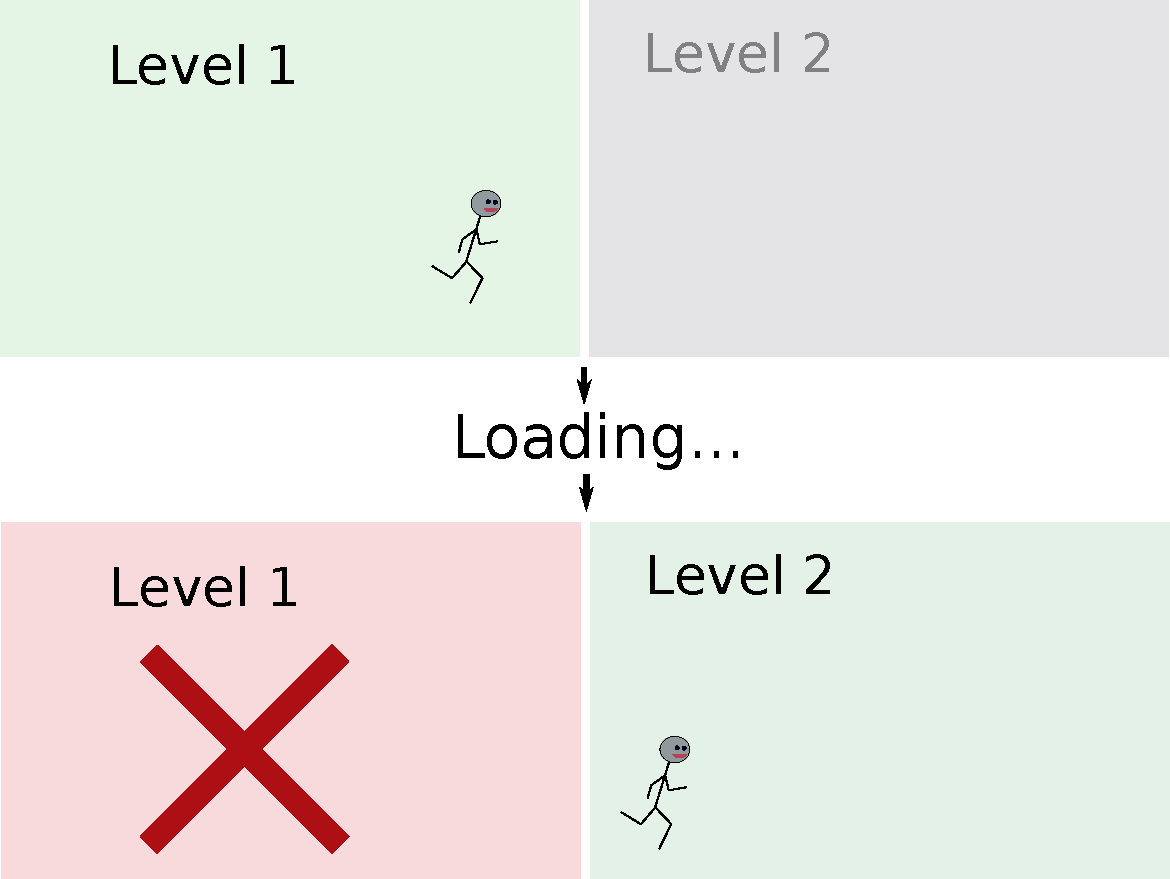
\includegraphics[scale=0.7]{level_loading_mechanics.pdf}
	\caption{Level loading mechanics}
	\label{fig:level_loading_mechanics}
\end{figure}

It is well know that computers(and other gaming devices) usually have two types of memory.
The first memory is the one we usually call main memory. Main memory is fast and slow.
The second memory is the secondary storage memory. This one is slow and big. Changing of level requires loading all the resources of the next level from secondary memory and, therefore, it is slow. That's why in most level-based games changing of level will pop-up a loading screen.and the player has to wait for a while.

\begin{figure}[H]
	\centering
	
\includegraphics[scale=0.7]{loading_sonic.png}
	\caption{One loading screen from \emph{Sonic}}
	\label{fig:loading_sonic}
\end{figure}

Some times the designers of the game use the loading screen to give tips to the player.

The approach used by level-based games is not useful for open world games we need world streaming in order to avoid loading screens.

\section{World streaming}

World streaming consists on loading game resources on demand. The concept is very similar to video streaming. In video streaming the data is sent from disk or from the network as it is needed. So in world streaming the game contents are taken from the disk (or from the network) to main memory as they are needed.
In contrast to video streaming, world streaming is not as straightforward. In video streaming the data is sequential, that is, you know what comes after. World streaming is different because what comes next depends on what the user does. So we must have the data prepared for all the decisions the user can make.
Imagine the case of platform game such as \emph{Terraria}. \emph{Terraria} is a 2D game that has an enormous map.

\begin{figure}[H]
	\centering
	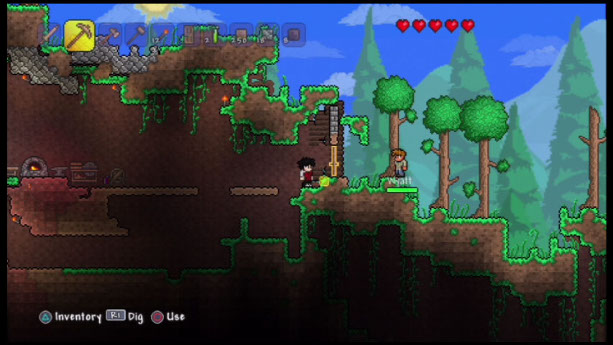
\includegraphics[scale=0.6]{terraria.jpg}
	\caption{Screenshot of \emph{Terraria}}
	\label{fig:terraria}
\end{figure}

In \emph{Terraria} the player can move in four directions (up, down, left, right). So when the user chooses to go to any of the four directions the data must be already prepared in main memory no mater what key is pressed.

\subsection{Examples of games using world streaming}

"Streaming is the backbone of everything we do. Everyone at the company understands how it's structured." said Adam Fowler, the Technical director at Rockstar North \cite{rockstar}.
Companies, such as Rockstar, know that world streaming is the technology that supports their success.

In this section we are going to show some of the most relevant games supported by the world streaming technology.

\paragraph{Hunter - Paul Holmes (1991)}

Hunter is one of the main influences of GTA (Grand Theft Auto). Hunter is a 3D action-adventure game in which the player could travel around a pretty big world. The degree of freedom in this game was enormous. There were many vehicles (bicycles, cars, ships, tanks, airplanes), places, and weapons. It is certainly not the first open world game but from the information we have I could affirm it might be the first game that used some kind of world streaming.

\begin{figure}[H]
	\centering
	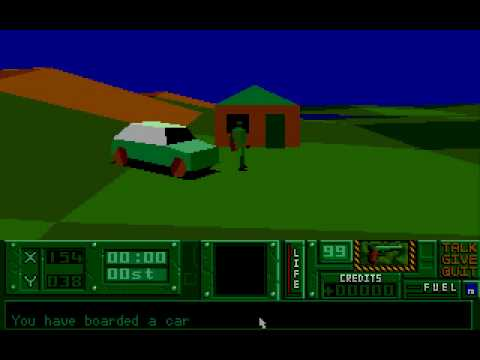
\includegraphics[scale=0.7]{hunter.jpg}
	\caption{Screenshot of \emph{Hunter}}
	\label{fig:hunter}
\end{figure}

In this game there were missions that could be completed but it was the player who decided whether or not to complete them.

Hunter was released for Amiga and Atari. The acceptance of the game was great and magazines ranked it with high scores.


\paragraph{Grand Theft Auto - Tarantula Studios (1997)}

This was the first Grand Theft Auto. With an enormous city and \emph{mainly} 2D graphics, GTA was the one that started the famous series of violent games. The player takes the role of a criminal that can drive all around the city without loading screens.

\begin{figure}[H]
	\centering
	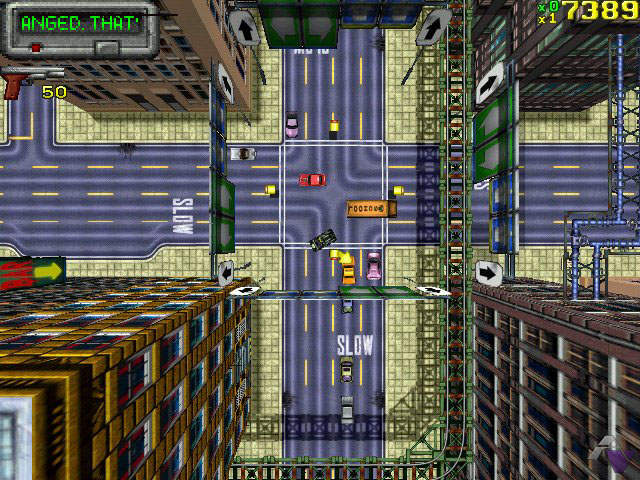
\includegraphics[scale=0.8]{gta.jpg}
	\caption{Screenshot of \emph{GTA}}
	\label{fig:gta}
\end{figure}

The game was released in 1997 for PC and PlayStation, and in 1998 for GameBoy Color. The GBC (GameBoy Color) version is considered to be a great technological achievement due to the hardware limitations of the portable console. The first GTA was successful in sells mainly thanks to the GBC version but magazines and users rated it low\cite{gta1}.


\paragraph{Midnight Club: Street Racing - Angel Studios (2000)}

Midnight Club is a series of open world racing games. In this game you take the role of an urban street racer. The player can drive all around \emph{The Big Apple} and challenge other street racers. In the missions you will have to defeat your enemies and scape from the cops. Completing missions will provide you respect and money to buy new cars. But you can skip missions and just enjoy driving around New York.

\begin{figure}[H]
	\centering
	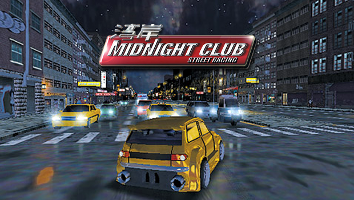
\includegraphics[scale=1]{midnight1.png}
	\caption{Screenshot of \emph{Midnight Club: Street Racing}}
	\label{fig:midnight1}
\end{figure}

This first Midnight Club was released in the same year that the PS2 (PlayStation 2) was commercialised. The acceptance of the public was good but sells were less than expected. One year later they released the GBA (GameBoy Advance) version which was rated poorly. Despite of its unfortunate sales this game is the one that started a successful saga.

\paragraph{Dungeon Siege - Gas Powered Games (2002)}

Dungeon Siege is a role-playing videogame very similar to \emph{Diablo} series. Scott Bilas, one of the developers of the game, published a very inspiring article about how the team managed to develop a game with such a big world\cite{worldbilas}. Thats to its flexible scripting engine the community was able to make modifications of the game, and even some people used the engine to make their own game. Despite the main story of the game is very linear there are many secondary missions and the player has quite freedom to move around. The greatest achievement of this game was avoiding all loading screens except for the initial one. Even taking portals is instantaneous. Graphics were impressive for the time being.

\begin{figure}[H]
	\centering
	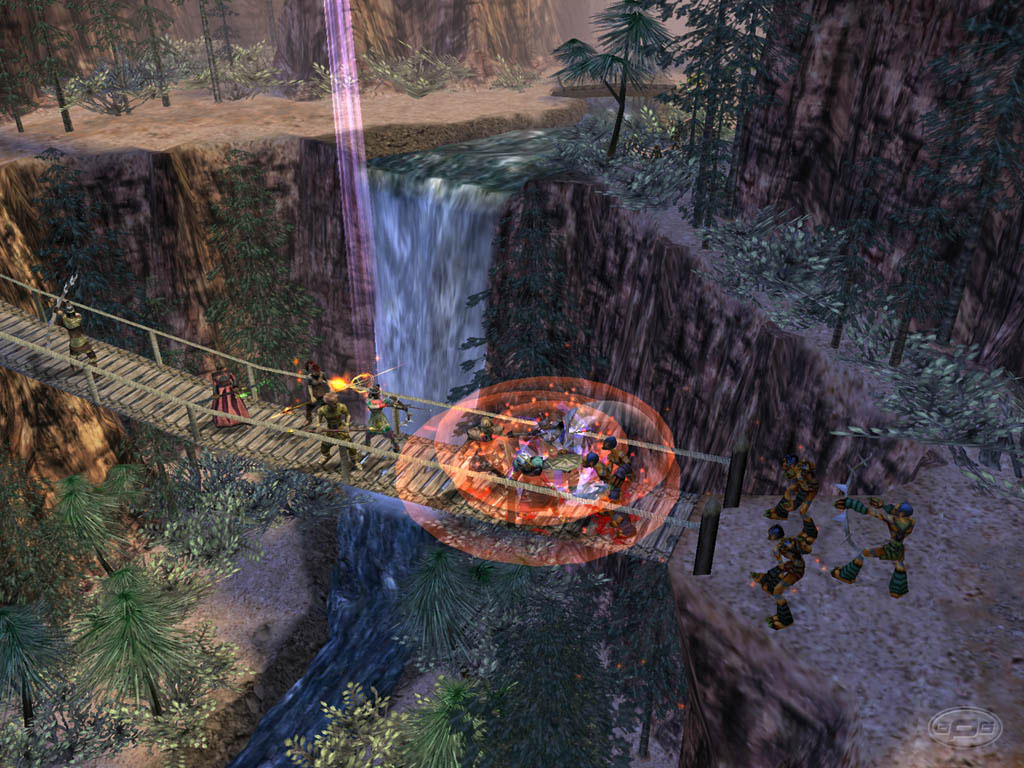
\includegraphics[scale=0.75]{dungeon_siege_screenshot.jpg}
	\caption{Screenshot of \emph{Dungeon Siege}}
	\label{fig:dungeonsiege1}
\end{figure}

Dungeon Siege had an online mode too. In the online mode you could grab your friends and complete the adventure in company.

Dungeon Siege had good sales but maybe not as much as it deserved for its technological quality and good graphics design

\paragraph{Grand Theft Auto: San Andreas - Rockstar North (2004)}

After the \emph{Rockstar}'s successful titles \emph{GTA III} and \emph{GTA: Vice City}, it came an even more sold game: \emph{GTA: San Andreas}. Take the role of \emph{Carl Johnson}, the feared gangster. This game has one of the biggest maps in the history of videogames. There is complete freedom to wander around any of the tree enormous cities.

\begin{figure}[H]
	\centering
	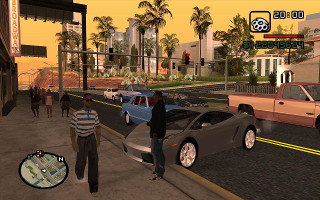
\includegraphics[scale=1]{sanan.jpg}
	\caption{Screenshot of \emph{GTA: San Andreas}}
	\label{fig:sanan}
\end{figure}

\emph{San Andreas} is the most sold PS2 game ever. Very successful for the PC and XBOX platforms too. And not only that, the game is still having good sales for PC and Android.

\paragraph{World Of Warcraft - Blizzard (2004)}

\emph{World of Warcraft} (\emph{WoW}) is an MMORPG (massively multiplayer online role-playing game). This game has a different type of world streaming from the one we have seen so far. In this case the information that provides the status of the entities doesn't come from the hard disk but from the network. World streaming in the network is even more challenging but, for instance, resource management is very similar. This has a big world and social interaction among players. Chatting, trading and fighting with other players is possible in \emph{WoW}.


\begin{figure}[H]
	\centering
	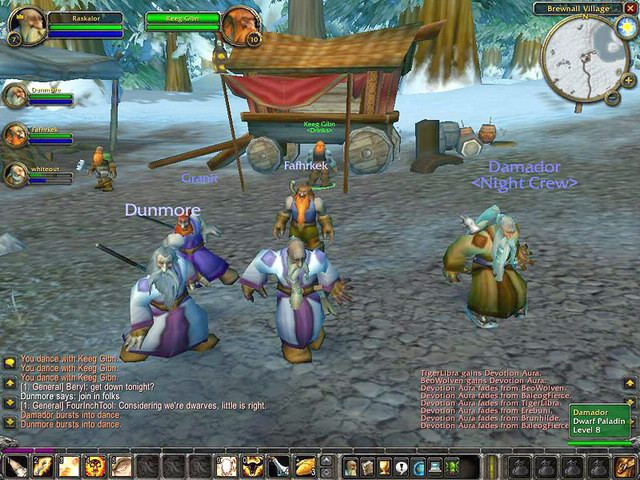
\includegraphics[scale=0.6]{wow.jpg}
	\caption{Screenshot of \emph{World of Warcraft}}
	\label{fig:wow}
\end{figure}

WoW has been the most played multiplayer game for many years and it is the game that provided most earnings of all times(\$10 billion)\cite{earnings}.

\paragraph{Fallout 3 - Bethesda Softworks (2008)}

World streaming is a feature present in many of the new-generation videogames. Fallout is just one of them that has an enormous world and impressive graphics.

\begin{figure}[H]
	\centering
		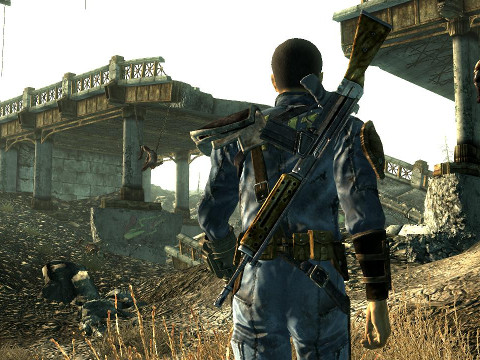
\includegraphics[scale=0.8]{fallout.jpeg}
	\caption{Screenshot of \emph{Fallout 3}}
	\label{fig:fallout}
\end{figure}


\paragraph{Minecraft - Mojang (2011)}

\emph{Minecraft} is the sandbox MMO that proved that games are not all about graphics.

\begin{figure}[H]
	\centering
	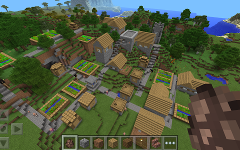
\includegraphics[scale=1]{minecraft.png}
	\caption{Screenshot of \emph{Minecraft}}
	\label{fig:minecraft}
\end{figure}

\emph{Minecraft} is the most sold PC game of all times.


\paragraph{Conclusion}

We have seen many games supported by the world streaming technology. The trend shows that open world games are becoming more popular and it does not seem it is going to stop.

\subsection{The strategy}

The most valuable source of information I have found about world streaming is an article called \emph{The Continuous World of Dungeon Siege} by \emph{Scott Bilas}\cite{worldbilas}. In this article, \emph{Scott Bilas} explains how they developed \emph{Dungeon Siege}. \emph{Dungeon Siege} is an open world 3D game released in 2002. It was developed by \emph{Gas Powered Games} and distributed by \emph{Microsoft}. In this article I have found many useful tips for implementing an open world streaming engine. \emph{Dungeon Siege} is a 3D game but you can only move in four directions (the world is landscape shaped). So the approach followed in \emph{Dungeon Siege} is similar to the one we would follow in a 2D game.

In \emph{Dungeon Siege} the world is divided into pieces of land which are aligned to a grid. These rectangles of land are called nodes. Any node can be connected to every other node. If two nodes are linked, that means that if the player is in one of them, he could travel to the other at any moment. Therefore, when the player is in one node we must be loading at least all the directly connected nodes. Normally the connections will match the adjacent pieces of land.

\begin{figure}[H]
	\centering
	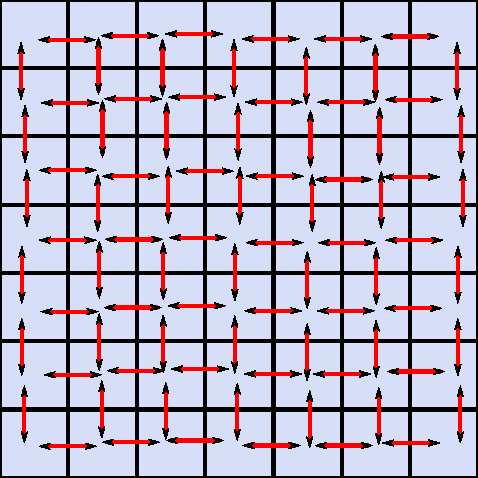
\includegraphics[scale=1]{connections.pdf}
	\caption{Connections of adjacent pieces of land (we are not taking into account the diagonals)}
	\label{fig:connections}
\end{figure}

But there are cases in which two adjacent nodes could not be connected (e.g. there is a wall separating them). Or there could be nodes that are connected and are not adjacent (e.g. there is a portal that will teleport the player from one place to another).


\begin{figure}[H]
	\centering
	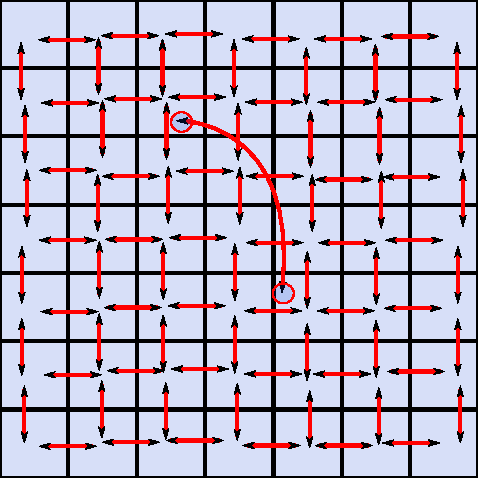
\includegraphics[scale=1]{connections2.pdf}
	\caption{Two nodes connected by a portal.}
	\label{fig:connections2}
\end{figure}

This node-based approach is the one used in Dungeon siege. The designers of the game used a custom tool that would allow to manage the connections of the nodes.

For our engine we are going to take a simpler approach and we will assume each node is connected to all the surrounding nodes (i.e 8 nodes at most). This will simplify the job of the designers of the game. With our approach taking portals will require a loading screen (which is very common current games).

\subsection{Loading Resources is slow}

Imagine that we have implemented our strategy and in a given moment the player has changed of node. We will have to load to main memory all the entities that are located in the new adjacent cell (or node). That implies: loading from disk the file that describes that cell, parsing that file in order to find the entities, loading all the resources that are required by the entities and finally creating the entities. So when the node had been loaded you would realize that you have spent 1 second (or much more) and in this time you haven't rendered a single frame!. Therefore, we have to solve this in some way.

The bottleneck here is the access to disk. Access to disk blocks the CPU and requires some time. So most of the time, when loading a new cell, the CPU would be idle while it could be doing important tasks (e.g. physics simulation or rendering). The solution that is suggested in the article of \emph{Scott Bilas} (and the one we have followed) is to use a separate thread for loading resources from disk. So if our main thread (the one that executes the main loop) needs to load a resource, instead of doing it itself, it asks the background thread to do it. This way, the main thread is never idle when there is job to be done and the secondary thread will be loading from disk at its own pace.

\begin{figure}[H]
	\centering
	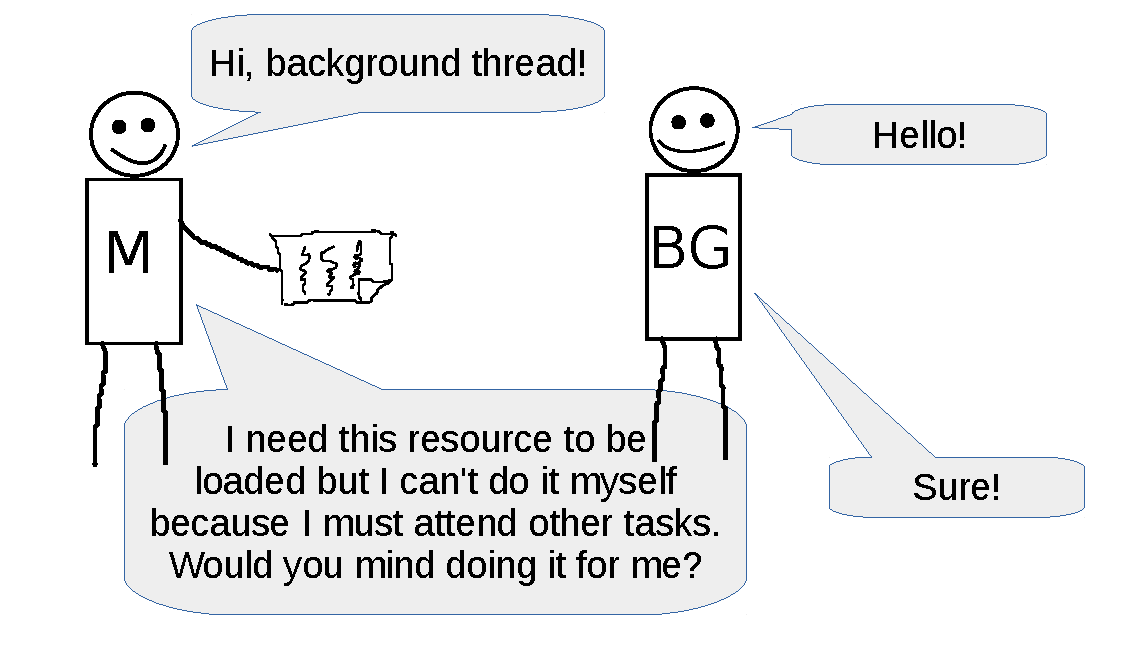
\includegraphics[scale=0.7]{comic1.pdf}
	\caption{Two threads talking.}
	\label{fig:comic1}
\end{figure}

\bibliography{tfg}

\begin{thebibliography}{99}

\bibitem{bestselling}
	\hypertarget{bestselling}
	List of the best-selling videogames.
	\newline
	\url{http://en.wikipedia.org/wiki/List_of_best-selling_video_games#All_platforms}
	
\bibitem{worldbilas}
	\hypertarget{worldbilas}
	The Continuous World of Dungeon Siege - Scott Bilas.
	\newline
	\url{http://scottbilas.com/files/2003/gdc_san_jose/continuous_world_paper.pdf}
	
\bibitem{rockstar}
	\hypertarget{rockstar}
	Technical leads Adam Fowler and Phil Hooker take us through the technology powering GTA V.
	\newline
	\url{http://www.develop-online.net/studio-profile/inside-rockstar-north-part-3-the-tech/0184140}
	
\bibitem{gta1}
	\hypertarget{gta1}
	GTA article at Wikipedia.
	\newline
	\url{http://en.wikipedia.org/wiki/Grand_Theft_Auto_%28video_game%29}
		

\bibitem{earnings}
\hypertarget{earnings}
Top 10 highest grossing videogames of all time.
\newline
\url{http://www.businessinsider.com/here-are-the-top-10-highest-grossing-video-games-of-all-time-2012-6?op=1}
	
\end{thebibliography}


\end{document}

